% !TEX program = xelatex
% Расчётно-графическая работа по дисциплине
% «Управление распределёнными системами», вариант 16.
% Сборка: latexmk main.tex (движок xelatex задан в .latexmkrc)
% ============================================================
% Преамбула (ГОСТ 7.32-2017, XeLaTeX)
% Перенесена из курсовой работы по ТАУ; добавлен TikZ для схем
% ============================================================
\documentclass[a4paper,14pt]{extreport}

% --- Шрифты и язык (XeLaTeX) --------------------------------
\usepackage{fontspec}
\setmainfont{Times New Roman}
\usepackage{polyglossia}
\setmainlanguage{russian}
\setotherlanguage{english}
% Моноширинный шрифт с поддержкой кириллицы (для \texttt)
\setmonofont{Courier New}
\newfontfamily\cyrillicfonttt{Courier New}

% --- Геометрия страницы -------------------------------------
\usepackage[
  left   = 30mm,
  right  = 15mm,
  top    = 20mm,
  bottom = 20mm
]{geometry}

% --- Межстрочный интервал и абзацный отступ -----------------
\usepackage{setspace}
\onehalfspacing
\setlength{\parindent}{1.25cm}

% --- Математика ----------------------------------------------
\usepackage{amsmath}
\usepackage{amssymb}
% Знаки нестрогих неравенств в принятом в русской литературе начертании
\renewcommand{\le}{\leqslant}
\renewcommand{\ge}{\geqslant}
% Сквозная нумерация формул (как в образце оформления)
\counterwithout{equation}{chapter}
% ГОСТ 7.32-2017, п. 6.8.1: отбивка формулы одинакова после полной
% и неполной строки
\makeatletter
\g@addto@macro\normalsize{%
  \setlength{\abovedisplayshortskip}{\abovedisplayskip}%
  \setlength{\belowdisplayshortskip}{\belowdisplayskip}}
\makeatother
\normalsize

% --- Рисунки и таблицы --------------------------------------
\usepackage{graphicx}
\graphicspath{{figures/}}
\usepackage{float}

\usepackage{booktabs}
\usepackage{longtable}
\usepackage{array}

% --- Подписи (ГОСТ: «Рисунок N — ...», «Таблица N — ...») ---
\usepackage{caption}
\DeclareCaptionLabelFormat{gost}{#1~#2}
\DeclareCaptionLabelSeparator{gost}{ --- }
\captionsetup{
  labelsep       = gost,
  labelformat    = gost,
  justification  = centering,
  skip           = 6pt
}
\captionsetup[figure]{
  name           = Рисунок,
  position       = below,
  justification  = centering
}
\captionsetup[table]{
  name           = Таблица,
  position       = above,
  justification  = raggedright,
  singlelinecheck= false
}

% Сквозная нумерация рисунков и таблиц (как в образце оформления)
\counterwithout{figure}{chapter}
\counterwithout{table}{chapter}

% --- Стиль заголовков (titlesec, как в образце оформления) --
\usepackage{titlesec}

% Заголовок раздела: «N Название» — полужирный, кегль основного
% текста, без слова «Глава», с абзацного отступа (ГОСТ 7.32-2017, п. 6.2.1)
\titleformat{\chapter}[hang]
  {\normalfont\bfseries}{\thechapter}{1ex}{}
\titlespacing*{\chapter}{\parindent}{0pt}{14pt}

% Структурные заголовки (\chapter*: содержание, выводы,
% список литературы) — по центру, полужирные
\titleformat{name=\chapter,numberless}[block]
  {\normalfont\bfseries\filcenter}{}{0pt}{}
\titlespacing*{name=\chapter,numberless}{0pt}{0pt}{14pt}

% Подразделы — полужирные, «N.M Название» без точки после номера,
% с абзацного отступа
\titleformat{\section}[hang]
  {\normalfont\bfseries}{\thesection}{1ex}{}
\titlespacing*{\section}{\parindent}{14pt}{8pt}

\titleformat{\subsection}[hang]
  {\normalfont\bfseries}{\thesubsection}{1ex}{}
\titlespacing*{\subsection}{\parindent}{12pt}{6pt}

% Содержание (ГОСТ 7.32-2017, пп. 5.4.1, 6.13): отточие у каждой записи,
% записи разделов без полужирного и без дополнительных отбивок
\makeatletter
\renewcommand*{\l@chapter}{\@dottedtocline{0}{0pt}{1.5em}}
\makeatother

% --- Прочие пакеты ------------------------------------------
\usepackage{enumitem}
% Перечисления: с абзацного отступа, без дополнительных отбивок
% (ГОСТ 7.32-2017, п. 6.4.6)
\setlist{nosep}
\setlist[enumerate]{nosep, wide=\parindent, label=\arabic*)}
\usepackage{hyperref}
\hypersetup{
  colorlinks = true,
  linkcolor  = black,
  urlcolor   = black,
  citecolor  = black
}
% Стабилизирует файл закладок (main.out) — без него сборке не
% хватает проходов для схождения перекрёстных ссылок
\usepackage{bookmark}

% --- Схемы (TikZ) -------------------------------------------
\usepackage{tikz}
\usetikzlibrary{arrows.meta, calc, patterns}

% --- Математические сокращения ------------------------------
% Частные производные: \pd{T}{z}, \pdd{T}{z}
\newcommand{\pd}[2]{\dfrac{\partial #1}{\partial #2}}
\newcommand{\pdd}[2]{\dfrac{\partial^2 #1}{\partial #2^2}}
\DeclareMathOperator{\Div}{div}
\DeclareMathOperator{\Grad}{grad}

% Запрет «висячих» строк
\clubpenalty=10000
\widowpenalty=10000
\displaywidowpenalty=10000

% Допуск на растяжение пробелов: строки с формулами не выходят на поле
\setlength{\emergencystretch}{2em}

\begin{document}
\begin{titlepage}
\thispagestyle{empty}
\centering

{Министерство науки и высшего образования Российской Федерации\\
федеральное государственное автономное образовательное учреждение\\
высшего образования\\
«Санкт-Петербургский политехнический университет Петра Великого»\\
(ФГАОУ ВО СПбПУ)\par}

\medskip

{Институт компьютерных наук и кибербезопасности\\
Высшая школа компьютерных технологий и информационных систем\par}

\vfill

{\bfseries РАСЧЁТНО-ГРАФИЧЕСКАЯ РАБОТА\par}
\medskip
{По дисциплине «Управление распределёнными системами»\par}
\medskip
{\bfseries Стационарное распределение температуры\\
в цилиндре с теплоизолированными торцами\par}
\medskip
{Вариант~16\par}

\vfill

\raggedright
\newcommand{\sigline}{%
  \begin{tabular}[t]{@{}c@{}}
    \makebox[5cm]{\hrulefill}\\[-0.6em]
    {\itshape\small <подпись>}
  \end{tabular}%
}

\begin{tabular}{@{}l@{\hspace{1.2cm}}c@{\hspace{1cm}}l@{}}
Выполнил:                  &           &                 \\
студент гр. 5130902/30201  & \sigline  & Р.\,В.~Садчев   \\[2.4em]
Проверила:                 &           &                 \\
преподаватель ВШКТиИС      & \sigline  & Н.\,В.~Сорокина
\end{tabular}

\medskip

\centering
«\rule[-0.2em]{1cm}{0.4pt}»~\rule[-0.2em]{3.5cm}{0.4pt}~2026~г.

\vfill

{Санкт-Петербург\\
2026\par}

\end{titlepage}
\clearpage
% ГОСТ 7.32-2017, п. 6.3.1: титульный лист входит в общую нумерацию,
% номер на нём не ставится — следующая страница имеет номер 2
\setcounter{page}{2}

\renewcommand{\contentsname}{СОДЕРЖАНИЕ}
\tableofcontents
% ============================================================
% ch1.tex — 1 ПОСТАНОВКА ЗАДАЧИ
% ============================================================
\chapter{Постановка задачи}
\label{ch:task}

Расчётное задание (вариант~16) сформулировано так.

\emph{Найти стационарное распределение температуры в цилиндре радиуса~$a$
и высоты~$h$ с теплоизолированными торцами, если боковая поверхность
поддерживается при температуре}
\begin{equation}
\label{eq:task}
T\big|_{r=a}=
\begin{cases}
0,   & 0<z<c,\\[2pt]
T_0, & c\le z<h.
\end{cases}
\end{equation}

В условии~\eqref{eq:task} приняты обозначения: $T$~— температура, К;
$r$~— расстояние от точки до оси цилиндра, м; $z$~— координата вдоль оси
цилиндра, отсчитываемая от нижнего торца, м; $a$ и $h$~— радиус и высота
цилиндра, м; $c$~— высота, на которой температура боковой поверхности
меняется скачком, м ($0<c<h$); $T_0$~— заданная постоянная температура
верхней части боковой поверхности, К. Величины $a$, $h$, $c$ и $T_0$
считаются известными. Искомой величиной является температура~$T$ во всех
точках цилиндра. Схема задачи показана на рисунке~\ref{fig:cylinder}.

\begin{figure}[H]
  \centering
  % Рисунок 1 — цилиндр и условия на его поверхности
% Параметры эскиза: радиус эллипса rx, ry; высота H; уровень z = c
\begin{tikzpicture}[>={Stealth[length=2.6mm]}, line cap=round, line join=round]
  \def\rx{2.3}
  \def\ry{0.62}
  \def\H{5.2}
  \def\C{2.1}

  % --- боковая поверхность: верхняя часть (T = T_0) закрашена ---
  \fill[gray!28]
    (-\rx,\C) arc[start angle=180, end angle=360, x radius=\rx, y radius=\ry]
    -- (\rx,\H) arc[start angle=0, end angle=-180, x radius=\rx, y radius=\ry]
    -- cycle;

  % --- верхний торец (теплоизолирован) ---
  \fill[white] (0,\H) ellipse[x radius=\rx, y radius=\ry];
  \fill[pattern=north east lines, pattern color=black!55]
    (0,\H) ellipse[x radius=\rx, y radius=\ry];
  \draw[thick] (0,\H) ellipse[x radius=\rx, y radius=\ry];

  % --- образующие ---
  \draw[thick] (-\rx,0) -- (-\rx,\H);
  \draw[thick] ( \rx,0) -- ( \rx,\H);

  % --- нижний торец ---
  \draw[thick] (-\rx,0) arc[start angle=180, end angle=360, x radius=\rx, y radius=\ry];
  \draw[dashed] (-\rx,0) arc[start angle=180, end angle=0, x radius=\rx, y radius=\ry];

  % --- окружность z = c (линия скачка температуры) ---
  \draw[semithick] (-\rx,\C) arc[start angle=180, end angle=360, x radius=\rx, y radius=\ry];
  \draw[dashed] (-\rx,\C) arc[start angle=180, end angle=0, x radius=\rx, y radius=\ry];

  % --- ось z ---
  \draw[dash dot] (0,-1.1) -- (0,\H);
  \draw[->] (0,\H) -- (0,\H+1.25) node[right] {$z$};
  \fill (0,0) circle[radius=1.3pt] node[below left=-1pt] {$O$};

  % --- ось r и радиус a ---
  \draw[->] (0,0) -- (\rx+1.7,0) node[above] {$r$};
  \fill (\rx,0) circle[radius=1.3pt];
  \node[above right=-1pt] at (\rx,0) {$a$};

  % --- размеры c и h слева ---
  \draw[thin] (-\rx,0)  -- (-\rx-1.55,0);
  \draw[thin] (-\rx,\C) -- (-\rx-0.85,\C);
  \draw[thin] (-\rx,\H) -- (-\rx-1.55,\H);
  \draw[<->, thin] (-\rx-0.65,0) -- (-\rx-0.65,\C) node[midway, left] {$c$};
  \draw[<->, thin] (-\rx-1.35,0) -- (-\rx-1.35,\H) node[midway, left] {$h$};

  % --- подписи условий ---
  \node[anchor=west] at (\rx+0.55, 0.5*\C)       {$T=0$};
  \node[anchor=west] at (\rx+0.55, 0.5*\C+0.5*\H) {$T=T_0$};
  \draw[thin] (\rx+0.5, 0.5*\C) -- (\rx-0.55, 0.5*\C-0.25);
  \draw[thin] (\rx+0.5, 0.5*\C+0.5*\H) -- (\rx-0.55, 0.5*\C+0.5*\H-0.25);
  \fill (\rx-0.55, 0.5*\C-0.25) circle[radius=1pt];
  \fill (\rx-0.55, 0.5*\C+0.5*\H-0.25) circle[radius=1pt];

  \node[anchor=west] (top) at (\rx+0.55, \H+0.75) {$\pd{T}{z}=0$};
  \draw[thin] (top.west) -- (0.95, \H+0.12);
  \fill (0.95, \H+0.12) circle[radius=1pt];

  \node[anchor=west] (bot) at (\rx+0.55, -1.15) {$\pd{T}{z}=0$};
  \draw[thin] (bot.west) -- (0.95, -0.25);
  \fill (0.95, -0.25) circle[radius=1pt];
\end{tikzpicture}

  \caption{Цилиндр и условия на его поверхности}
  \label{fig:cylinder}
\end{figure}

Физический смысл задачи таков. Пусть для определённости $T_0>0$. Сплошной
цилиндр нагревается через верхнюю часть боковой поверхности, где
поддерживается температура~$T_0$, и охлаждается через нижнюю, температура
которой равна нулю. Через торцы тепло не проходит. Спустя достаточно
большое время температура в каждой точке цилиндра перестаёт меняться:
устанавливается стационарный тепловой режим. Распределение температуры
в этом режиме и требуется найти.

Нулевое значение температуры в условии~\eqref{eq:task} означает выбор начала
отсчёта: температура отсчитывается от её значения на нижней части боковой
поверхности. Если нижняя часть имеет температуру~$T_{\text{н}}$,
а верхняя~— $T_{\text{в}}$, то заменой искомой функции $T$ на разность
$T-T_{\text{н}}$ задача сводится к рассматриваемой
с $T_0=T_{\text{в}}-T_{\text{н}}$.

Разделы 1 и 2 отчёта соответствуют первому этапу расчётного задания: по
словесному описанию задачи дать её математическую постановку.
В соответствии с заданной структурой отчёта далее будут получены
аналитическое и численное решения задачи и выполнен анализ полученных
решений.
   % 1 Постановка задачи
% ============================================================
% ch2.tex — 2 МАТЕМАТИЧЕСКАЯ МОДЕЛЬ (этап 1)
% ============================================================
\chapter{Математическая модель}
\label{ch:model}

Математическая модель задачи состоит из дифференциального уравнения,
которому удовлетворяет температура внутри цилиндра, и условий на его
границе. Ниже перечислены принятые допущения, выведены уравнение и
граничные условия, записана математическая постановка задачи и рассмотрены
её свойства. При построении модели использованы материалы лекций курса
и учебная литература~[1--3].

\section{Принятые допущения}
\label{sec:assumptions}

Модель строится при следующих допущениях:
\begin{enumerate}
  \item цилиндр сплошной, его материал однороден и изотропен: коэффициент
        теплопроводности одинаков во всех точках и по всем направлениям,
        а также не зависит от температуры;
  \item внутри цилиндра нет источников и стоков тепла;
  \item тепло внутри цилиндра переносится только теплопроводностью;
  \item тепловой режим стационарный: температура в каждой точке не зависит
        от времени;
  \item торцы идеально теплоизолированы, а температура боковой поверхности
        в точности равна заданной и на высоте $z=c$ меняется скачком.
\end{enumerate}

\section{Уравнение стационарной теплопроводности}
\label{sec:heat}

Пусть $T(M,t)$~— температура в точке~$M$ тела в момент времени~$t$.
Перенос тепла теплопроводностью описывается законом Фурье~[2,\,3]:
\begin{equation}
\label{eq:fourier}
\vec q=-k\,\Grad T,
\postdisplaypenalty=10000
\end{equation}
где $\vec q$~— вектор плотности теплового потока, Вт/м$^2$;\\
\hphantom{где }$k$~— коэффициент теплопроводности, Вт/(м$\cdot$К).

Вектор~$\vec q$ направлен в сторону переноса тепла, а его модуль равен
количеству тепла, проходящему за единицу времени через единичную площадку,
перпендикулярную потоку. Знак «минус» показывает, что тепло переносится
в сторону убывания температуры.

Выделим внутри тела произвольный объём~$V$, ограниченный замкнутой
поверхностью~$S$ с внешней нормалью~$\vec n$, и запишем для него баланс
тепла за единицу времени:
\begin{equation}
\label{eq:balance}
\iiint\limits_V C\rho\,\pd{T}{t}\,dV
=-\iint\limits_S \vec q\cdot\vec n\,dS+\iiint\limits_V F\,dV,
\postdisplaypenalty=10000
\end{equation}
где $C$~— удельная теплоёмкость, Дж/(кг$\cdot$К);\\
\hphantom{где }$\rho$~— плотность, кг/м$^3$;\\
\hphantom{где }$F$~— мощность внутренних источников тепла в единице объёма,
Вт/м$^3$.

Левая часть равенства~\eqref{eq:balance}~— скорость изменения количества
тепла, запасённого в объёме~$V$. Первое слагаемое правой части~— тепло,
поступающее в объём через поверхность~$S$, второе~— тепло, выделяемое
источниками.

По формуле Остроградского поток вектора~$\vec q$ через замкнутую поверхность
равен интегралу от его расходимости по объёму:
\begin{equation}
\label{eq:ostrogradsky}
\iint\limits_S \vec q\cdot\vec n\,dS=\iiint\limits_V \Div\vec q\,dV .
\end{equation}
Заменяя по этой формуле поверхностный интеграл в~\eqref{eq:balance}
объёмным и подставляя закон Фурье~\eqref{eq:fourier}, получаем
\begin{equation}
\label{eq:balance-vol}
\iiint\limits_V\Bigl(C\rho\,\pd{T}{t}-\Div\bigl(k\,\Grad T\bigr)-F\Bigr)dV=0 .
\end{equation}
Объём~$V$ произволен, а подынтегральная функция непрерывна, поэтому она
равна нулю в каждой точке тела:
\begin{equation}
\label{eq:heat-general}
C\rho\,\pd{T}{t}=\Div\bigl(k\,\Grad T\bigr)+F .
\end{equation}

Для однородного тела $k=\mathrm{const}$ и
$\Div\bigl(k\,\Grad T\bigr)=k\,\Delta T$, где $\Delta$~— оператор Лапласа:
\begin{equation}
\label{eq:lap-cart}
\Delta T=\pdd{T}{x}+\pdd{T}{y}+\pdd{T}{z} .
\end{equation}
Из~\eqref{eq:heat-general} получаем уравнение теплопроводности
\begin{equation}
\label{eq:heat}
\pd{T}{t}=\chi\,\Delta T+\frac{F}{C\rho},
\qquad \chi=\frac{k}{C\rho},
\postdisplaypenalty=10000
\end{equation}
где $\chi$~— коэффициент температуропроводности, м$^2$/с. В лекциях курса
это уравнение записано в виде $u_t=a^2\Delta u+f$, то есть $\chi$
соответствует $a^2$, а $F/(C\rho)$~— функции~$f$. Буквы $a$ и $c$ в условии
задачи уже использованы (радиус цилиндра и высота, на которой температура
боковой поверхности меняется скачком), поэтому коэффициент
температуропроводности обозначен~$\chi$, а удельная теплоёмкость~— $C$.

Режим стационарный, поэтому $\partial T/\partial t=0$; источников тепла
нет, поэтому $F=0$. Уравнение~\eqref{eq:heat} переходит в уравнение Лапласа
\begin{equation}
\label{eq:laplace}
\Delta T=0 .
\end{equation}
Уравнение~\eqref{eq:laplace} не содержит характеристик материала $k$, $C$
и~$\rho$. Следовательно, стационарное распределение температуры
в однородном теле без внутренних источников определяется только формой тела
и условиями на его границе.

\section{Цилиндрические координаты и осевая симметрия}
\label{sec:cyl}

Границу цилиндра удобно описывать в цилиндрических координатах
$(r,\varphi,z)$, которые связаны с декартовыми координатами формулами
\begin{equation}
\label{eq:cyl}
x=r\cos\varphi,\qquad y=r\sin\varphi,\qquad z=z,
\postdisplaypenalty=10000
\end{equation}
где $r\ge 0$~— расстояние от точки до оси~$Oz$;\\
\hphantom{где }$\varphi$~— полярный угол, $0\le\varphi<2\pi$.

Ось~$Oz$ совпадает с осью цилиндра и направлена от нижнего торца
к верхнему, начало координат помещено в центр нижнего торца. В этих
координатах цилиндр занимает область
\begin{equation}
\label{eq:Omega}
\Omega=\bigl\{(r,\varphi,z):\ 0\le r<a,\ \ 0\le\varphi<2\pi,\ \ 0<z<h\bigr\},
\end{equation}
боковая поверхность задаётся уравнением $r=a$, а торцы~— уравнениями
$z=0$ и $z=h$.

Оператор Лапласа в цилиндрических координатах имеет вид~[3]
\begin{equation}
\label{eq:lap-cyl}
\Delta T=\frac{1}{r}\,\pd{}{r}\Bigl(r\,\pd{T}{r}\Bigr)
+\frac{1}{r^2}\,\pdd{T}{\varphi}+\pdd{T}{z} .
\end{equation}

Цилиндр~— тело вращения с осью~$Oz$, а условия на его поверхности не
зависят от угла~$\varphi$: заданная условием~\eqref{eq:task} температура
боковой поверхности зависит только от~$z$, торцы теплоизолированы целиком.
Ни одно значение угла~$\varphi$ не выделено, поэтому искомое температурное
поле осесимметрично:
\begin{equation}
\label{eq:axisym}
T=T(r,z),\qquad \pd{T}{\varphi}=0 .
\end{equation}
Строгое обоснование равенств~\eqref{eq:axisym} опирается на единственность
решения и приведено в подразделе~\ref{sec:type}.
Подставляя~\eqref{eq:lap-cyl} и~\eqref{eq:axisym} в уравнение
Лапласа~\eqref{eq:laplace}, получаем
\begin{equation}
\label{eq:main-div}
\frac{1}{r}\,\pd{}{r}\Bigl(r\,\pd{T}{r}\Bigr)+\pdd{T}{z}=0,
\end{equation}
или, после дифференцирования произведения,
\begin{equation}
\label{eq:main}
\pdd{T}{r}+\frac{1}{r}\,\pd{T}{r}+\pdd{T}{z}=0 .
\end{equation}
Задача стала двумерной. Функция $T(r,z)$ ищется в прямоугольнике
\begin{equation}
\label{eq:Pi}
\Pi=\bigl\{(r,z):\ 0<r<a,\ \ 0<z<h\bigr\},
\end{equation}
который представляет собой половину осевого сечения цилиндра.

\section{Граничные условия}
\label{sec:bc}

\emph{Боковая поверхность.} По условию боковая поверхность поддерживается
при заданной температуре, то есть в каждой её точке известно значение
искомой функции:
\begin{equation}
\label{eq:bc-side}
T(a,z)=\mu(z),\quad 0<z<h,
\qquad
\mu(z)=
\begin{cases}
0,   & 0<z<c,\\[2pt]
T_0, & c\le z<h .
\end{cases}
\end{equation}
Это граничное условие I~рода (условие Дирихле). Оно неоднородно, а функция
$\mu(z)$ кусочно-постоянна и имеет разрыв первого рода в точке $z=c$.

\emph{Торцы.} Количество тепла, проходящее за единицу времени через
единицу площади поверхности тела в направлении внешней нормали~$\vec n$,
в силу закона Фурье~\eqref{eq:fourier} равно
\begin{equation}
\label{eq:flux-n}
q_n=\vec q\cdot\vec n=-k\,\Grad T\cdot\vec n=-k\,\pd{T}{n} .
\end{equation}
Торец теплоизолирован, если тепло через него не проходит: $q_n=0$, то есть
$\partial T/\partial n=0$. На верхнем торце $z=h$ внешняя нормаль направлена
вдоль оси~$Oz$ и $\partial T/\partial n=\partial T/\partial z$. На нижнем
торце $z=0$ она направлена противоположно оси и
$\partial T/\partial n=-\partial T/\partial z$. В обоих случаях получаем
\begin{equation}
\label{eq:bc-ends}
\pd{T}{z}\bigg|_{z=0}=0,\qquad \pd{T}{z}\bigg|_{z=h}=0,\qquad 0\le r<a .
\end{equation}
Это однородные граничные условия II~рода (условия Неймана).

\emph{Ось цилиндра.} Отрезок $r=0$ не является частью поверхности
цилиндра: точки оси лежат внутри тела. Однако он служит стороной
прямоугольника~$\Pi$, а коэффициент $1/r$ уравнения~\eqref{eq:main} при
$r\to 0$ неограниченно растёт. У~этого уравнения есть решения, которые на
оси обращаются в бесконечность, например $T=A\ln(r/a)$, где $A\ne 0$~—
постоянная. Такое решение соответствует источнику или стоку тепла на оси,
а по принятым допущениям их нет. Поэтому на оси ставится условие
ограниченности
\begin{equation}
\label{eq:bc-axis}
\bigl|T(0,z)\bigr|<\infty,\qquad 0\le z\le h .
\end{equation}
Для осесимметричного поля, гладкого на оси, из симметрии следует также
равенство
\begin{equation}
\label{eq:bc-axis-n}
\pd{T}{r}\bigg|_{r=0}=0,
\end{equation}
которое удобно использовать при численном решении.

\section{Математическая постановка задачи}
\label{sec:statement}

До использования осевой симметрии задача ставится в трёхмерной
области~$\Omega$: требуется найти функцию $T(r,\varphi,z)$ из условий
\begin{equation}
\label{eq:problem3d}
\begin{cases}
\Delta T=0,
  & 0<r<a,\ \ 0\le\varphi<2\pi,\ \ 0<z<h,\\[6pt]
\pd{T}{z}\bigg|_{z=0}=0,\qquad \pd{T}{z}\bigg|_{z=h}=0,
  & 0\le r<a,\ \ 0\le\varphi<2\pi,\\[10pt]
T\big|_{r=a}=\mu(z),
  & 0\le\varphi<2\pi,\ \ 0<z<h,\\[6pt]
\bigl|T\big|_{r=0}\bigr|<\infty,
  & 0\le z\le h,\\[6pt]
T(r,\varphi+2\pi,z)=T(r,\varphi,z),
  & 0<r\le a,\ \ 0\le z\le h,
\end{cases}
\postdisplaypenalty=10000
\end{equation}
где оператор Лапласа имеет вид~\eqref{eq:lap-cyl}, а последнее условие~—
условие периодичности по углу: значениям $\varphi$ и $\varphi+2\pi$
отвечает одна и та же точка. Граничные условия
задачи~\eqref{eq:problem3d} не зависят от~$\varphi$, поэтому её решение
осесимметрично: слагаемое с $\partial^2T/\partial\varphi^2$ исчезает,
условие периодичности выполняется автоматически, и задача сводится
к двумерной.

Объединяя уравнение~\eqref{eq:main} с условиями
\eqref{eq:bc-side}, \eqref{eq:bc-ends}, \eqref{eq:bc-axis}, приходим
к итоговой постановке. Требуется найти функцию $T(r,z)$, дважды непрерывно
дифференцируемую в прямоугольнике~$\Pi$ и удовлетворяющую условиям
\begin{equation}
\label{eq:problem}
\begin{cases}
\pdd{T}{r}+\dfrac{1}{r}\,\pd{T}{r}+\pdd{T}{z}=0,
  & 0<r<a,\ \ 0<z<h,\\[10pt]
\pd{T}{z}\bigg|_{z=0}=0,\qquad \pd{T}{z}\bigg|_{z=h}=0,
  & 0\le r<a,\\[10pt]
T\big|_{r=a}=\mu(z),
  & 0<z<h,\\[6pt]
\bigl|T\big|_{r=0}\bigr|<\infty,
  & 0\le z\le h,
\end{cases}
\end{equation}
где $T(r,z)$~— искомая функция;\\
\hphantom{где }$a$, $h$, $c$, $T_0$~— заданные параметры;\\
\hphantom{где }$\mu(z)$~— известная функция: $\mu(z)=0$ при
\mbox{$0<z<c$} и $\mu(z)=T_0$ при \mbox{$c\le z<h$}
(формула~\eqref{eq:bc-side}).

В лекциях курса решение краевой задачи ищется в классе функций, дважды
непрерывно дифференцируемых в области и непрерывных в замкнутой области.
В задаче~\eqref{eq:problem} граничная функция~$\mu(z)$ разрывна, и решение
не может быть непрерывным в точке $(a,c)$. Поэтому вместо непрерывности
в замкнутой области от него требуются ограниченность в области~$\Pi$
и непрерывность вплоть до границы всюду, кроме этой точки. Значение
функции~$\mu$ в самой точке $z=c$ на решение не влияет. Чтобы условия на
торцах имели смысл, производная $\partial T/\partial z$ должна быть
непрерывна вплоть до отрезков $z=0$ и $z=h$, $0\le r<a$.

В лекциях граница области предполагается гладкой, а граница цилиндра лишь
кусочно-гладкая: на рёбрах $r=a$, $z=0$ и $r=a$, $z=h$ нормаль не
определена. Поэтому условия~\eqref{eq:bc-ends} поставлены при $r<a$,
условие~\eqref{eq:bc-side}~— при $0<z<h$, а на самих рёбрах условия не
задаются. Расчётная область и условия на её границе показаны на
рисунке~\ref{fig:domain}.

\begin{figure}[H]
  \centering
  % Рисунок 2 — расчётная область (меридиональное сечение цилиндра)
\begin{tikzpicture}[>={Stealth[length=2.6mm]}, line cap=round, line join=round]
  \def\A{5.6}
  \def\H{6.2}
  \def\C{2.5}

  % --- теплоизоляция торцов (штриховка снаружи области) ---
  \fill[pattern=north east lines, pattern color=black!55] (0,-0.28) rectangle (\A,0);
  \fill[pattern=north east lines, pattern color=black!55] (0,\H) rectangle (\A,\H+0.28);

  % --- область ---
  \fill[gray!10] (0,0) rectangle (\A,\H);
  \draw[very thick] (0,0) -- (\A,0);
  \draw[very thick] (0,\H) -- (\A,\H);
  \draw[very thick] (\A,0) -- (\A,\C);
  \draw[line width=2.2pt, gray!70!black] (\A,\C) -- (\A,\H);
  \draw[dash dot, thick] (0,0) -- (0,\H);

  % --- оси ---
  \draw[->] (0,\H) -- (0,\H+1.35) node[left] {$z$};
  \draw[->] (\A,0) -- (\A+1.9,0) node[below] {$r$};
  \draw[dash dot] (0,0) -- (0,-0.9);

  % --- отметки ---
  \node[below left=-1pt] at (0,0) {$O$};
  \node[below=6pt] at (\A,0) {$a$};
  \draw[thin] (-0.12,\C) -- (0.12,\C);
  \node[left=3pt] at (0,\C) {$c$};
  \node[left=3pt] at (0,\H) {$h$};
  \draw[thin, dashed] (0,\C) -- (\A,\C);
  \fill (\A,\C) circle[radius=2pt];

  % --- уравнение внутри области ---
  \node at (0.5*\A, 0.5*\C+0.5*\H+0.25)
    {$\dfrac{1}{r}\,\pd{}{r}\!\Bigl(r\,\pd{T}{r}\Bigr)+\pdd{T}{z}=0$};
  \node at (0.5*\A, 0.5*\C) {$\Pi$};

  % --- граничные условия ---
  \node[below] at (0.5*\A,-0.32) {$\pd{T}{z}=0$};
  \node[above] at (0.5*\A,\H+0.3) {$\pd{T}{z}=0$};
  \node[right=4pt] at (\A, 0.5*\C+0.2) {$T=0$};
  \node[right=4pt] at (\A, 0.5*\C+0.5*\H) {$T=T_0$};
  \node[left=4pt] at (0, 0.5*\C+0.5*\H+0.25) {$|T|<\infty$};

  % --- внешние нормали к поверхности цилиндра ---
  \draw[->, thick] (0.78*\A,\H) -- (0.78*\A,\H+0.95) node[right] {$\vec n$};
  \draw[->, thick] (0.78*\A,0) -- (0.78*\A,-0.95) node[right] {$\vec n$};
  \draw[->, thick] (\A,0.9*\H) -- (\A+0.95,0.9*\H) node[above] {$\vec n$};
\end{tikzpicture}

  \caption{Расчётная область и граничные условия}
  \label{fig:domain}
\end{figure}

\section{Тип уравнения и свойства задачи}
\label{sec:type}

\emph{Тип уравнения.} Уравнение~\eqref{eq:main}~— линейное однородное
уравнение второго порядка с двумя независимыми переменными $r$ и~$z$.
Сравним его с общим видом уравнения, линейного относительно старших
производных~[2], записанным для независимых переменных $r$, $z$ и искомой
функции~$T$:
\begin{equation}
\label{eq:general}
a_{11}\,\pdd{T}{r}+2a_{12}\,\frac{\partial^2 T}{\partial r\,\partial z}
+a_{22}\,\pdd{T}{z}+\Phi\Bigl(r,z,T,\pd{T}{r},\pd{T}{z}\Bigr)=0 .
\end{equation}
Для уравнения~\eqref{eq:main} $a_{11}=1$, $a_{12}=0$, $a_{22}=1$,
$\Phi=(1/r)\,\partial T/\partial r$ (коэффициенты $a_{11}$, $a_{12}$,
$a_{22}$ не связаны с радиусом цилиндра~$a$). Тогда
\begin{equation}
\label{eq:discr}
D=a_{12}^2-a_{11}a_{22}=-1<0,
\end{equation}
и уравнение~\eqref{eq:main} относится к эллиптическому типу во всей
области~$\Pi$. Слагаемое с первой производной на тип уравнения не влияет.

Величина~$D$~— дискриминант характеристического уравнения
$a_{11}\,dz^2-2a_{12}\,dr\,dz+a_{22}\,dr^2=0$. Для
уравнения~\eqref{eq:main} оно имеет вид $dz^2+dr^2=0$ и вещественных решений
не имеет. Значит, вещественных характеристик у уравнения~\eqref{eq:main}
нет, а его старшая часть~— сумма вторых производных по $r$ и по~$z$~— уже
записана в каноническом виде. Исходное уравнение Лапласа~\eqref{eq:laplace}
с тремя независимыми переменными также относится к эллиптическому типу: все
коэффициенты его характеристической квадратичной формы
$\lambda_1^2+\lambda_2^2+\lambda_3^2$ отличны от нуля и имеют один знак.

\emph{Тип задачи.} Время в уравнение не входит, начальных условий нет,
поэтому~\eqref{eq:problem}~— краевая задача. На разных частях границы
заданы условия разного рода: на боковой поверхности~— I~рода, на торцах~—
II~рода. При этом задача не является смешанной в том смысле, который принят
в курсе лекций: смешанной там называется начально-краевая задача. Уравнение
и условия на торцах однородны, единственная неоднородность задачи~—
функция~$\mu(z)$ в условии на боковой поверхности.

\emph{Единственность решения.} Пусть $T_1$ и $T_2$~— два решения
трёхмерной задачи~\eqref{eq:problem3d}. Их разность $w=T_1-T_2$
удовлетворяет уравнению Лапласа $\Delta w=0$ в области~$\Omega$, условию
${w=0}$ на боковой поверхности и условию ${\partial w/\partial n=0}$ на
торцах. Так как
$\Div(w\,\Grad w)=|\Grad w|^2+w\,\Delta w=|\Grad w|^2$, формула
Остроградского~\eqref{eq:ostrogradsky} для вектора $w\,\Grad w$ и
области~$\Omega$ даёт
\begin{equation}
\label{eq:energy}
\iiint\limits_{\Omega}|\Grad w|^{2}\,dV
=\iint\limits_{S_\Omega} w\,\pd{w}{n}\,dS=0,
\end{equation}
где $S_\Omega$~— поверхность цилиндра. Поверхностный интеграл равен нулю,
потому что на боковой поверхности ${w=0}$, а на торцах
${\partial w/\partial n=0}$. Подынтегральная функция слева неотрицательна,
поэтому $\Grad w=0$ всюду в~$\Omega$, то есть $w=\mathrm{const}$, а из
условия на боковой поверхности следует ${w\equiv 0}$. Значит,
$T_1\equiv T_2$: задача~\eqref{eq:problem3d} не может иметь двух различных
решений. Тем самым единственно и решение двумерной
задачи~\eqref{eq:problem}: каждое её решение~— это не зависящее
от~$\varphi$ решение задачи~\eqref{eq:problem3d}.

Равенство~\eqref{eq:energy} справедливо, если первые производные
функции~$w$ ограничены вплоть до поверхности цилиндра. В рассматриваемой
задаче функция~$\mu(z)$ разрывна, и о решениях $T_1$ и $T_2$ вблизи
окружности $r=a$, $z=c$ известно лишь то, что они ограничены;
ограниченность производных их разности заранее не гарантирована. В этом
случае единственность ограниченного решения доказывается с помощью принципа
максимума, так же как для первой краевой задачи с разрывными граничными
значениями~[2].

Из единственности следует осевая симметрия~\eqref{eq:axisym}. Коэффициенты
оператора~\eqref{eq:lap-cyl} и граничные условия не зависят от~$\varphi$,
поэтому вместе с функцией $T(r,\varphi,z)$ решением
задачи~\eqref{eq:problem3d} при любом~$\alpha$ является и функция
$T(r,\varphi+\alpha,z)$. Решение единственно, значит, обе функции
совпадают, и $T$ не зависит от~$\varphi$.

\emph{Границы значений температуры.} По принципу максимума~[2,\,3] функция,
удовлетворяющая уравнению Лапласа и отличная от постоянной, не принимает
наибольшего и наименьшего значений во внутренних точках области. На торцах
цилиндра экстремум также невозможен. Условия~\eqref{eq:bc-ends} позволяют
продолжить решение чётным образом через плоскость $z=0$:
$T(r,-z)=T(r,z)$. Продолженная функция удовлетворяет уравнению Лапласа
в цилиндре $-h<z<h$ и принимает те же значения, что и исходная, а точки
торца $z=0$ для неё внутренние. Так же рассматривается торец $z=h$. Поэтому
наибольшее и наименьшее значения температуры определяются её значениями на
боковой поверхности, и при $T_0>0$
\begin{equation}
\label{eq:bounds}
0\le T(r,z)\le T_0 .
\end{equation}
Разрыв функции~$\mu(z)$ оценку~\eqref{eq:bounds} не нарушает: для
ограниченных решений она сохраняется~[2].

Из принципа максимума следует также устойчивость решения: если граничную
функцию~$\mu(z)$ изменить не более чем на~$\varepsilon$, то решение
изменится не более чем на~$\varepsilon$. Существование решения
показано в разделе~\ref{ch:analytic}: решение построено в явном виде
методом функции Грина.

\section{Безразмерная форма задачи}
\label{sec:dimless}

Введём безразмерные переменные
\begin{equation}
\label{eq:dimless-vars}
\xi=\frac{r}{a},\qquad \zeta=\frac{z}{h},\qquad \theta=\frac{T}{T_0} .
\end{equation}
Тогда $\partial/\partial r=(1/a)\,\partial/\partial\xi$,
$\partial/\partial z=(1/h)\,\partial/\partial\zeta$, и после умножения
уравнения~\eqref{eq:main-div} на $a^2/T_0$ задача~\eqref{eq:problem}
принимает вид
\begin{equation}
\label{eq:dimless}
\begin{cases}
\dfrac{1}{\xi}\,\pd{}{\xi}\Bigl(\xi\,\pd{\theta}{\xi}\Bigr)
+\Bigl(\dfrac{a}{h}\Bigr)^{2}\pdd{\theta}{\zeta}=0,
  & 0<\xi<1,\ \ 0<\zeta<1,\\[10pt]
\pd{\theta}{\zeta}\bigg|_{\zeta=0}=0,\qquad
\pd{\theta}{\zeta}\bigg|_{\zeta=1}=0,
  & 0\le\xi<1,\\[10pt]
\theta\big|_{\xi=1}=\mu_0(\zeta),
  & 0<\zeta<1,\\[6pt]
\bigl|\theta\big|_{\xi=0}\bigr|<\infty,
  & 0\le\zeta\le 1,
\end{cases}
\postdisplaypenalty=10000
\end{equation}
где $\mu_0(\zeta)=\mu(h\zeta)/T_0$~— безразмерная температура боковой
поверхности: $\mu_0=0$ при \mbox{$0<\zeta<c/h$} и $\mu_0=1$ при
\mbox{$c/h\le\zeta<1$}.

В задачу~\eqref{eq:dimless} входят только два безразмерных параметра~—
отношение радиуса цилиндра к его высоте $a/h$ и относительная высота линии
скачка температуры $c/h$; они и определяют форму температурного поля.
Температура~$T_0$ служит масштабом:
\begin{equation}
\label{eq:scaling}
T(r,z)=T_0\,\theta\Bigl(\frac{r}{a},\frac{z}{h}\Bigr).
\end{equation}
   % 2 Математическая модель            (этап 1)
% ============================================================
% ch3.tex — 3 АНАЛИТИЧЕСКОЕ РЕШЕНИЕ (этап 2)
% ============================================================
\chapter{Аналитическое решение}
\label{ch:analytic}

Аналитическое решение задачи строится методом функции Грина. Сначала
решение трёхмерной задачи~\eqref{eq:problem3d} выражается через функцию
Грина интегралом по боковой поверхности цилиндра. Затем функция Грина
находится в виде ряда по собственным функциям задач Штурма--Лиувилля по
переменным $z$ и~$\varphi$; коэффициенты ряда определяются из
обыкновенного дифференциального уравнения по~$r$. В конце интеграл
вычисляется, и температура выражается через все параметры задачи.
Использованы материалы лекций курса и литература~[1,\,2,\,4].

\section{Функция Грина и интегральное представление решения}
\label{sec:green-def}

\emph{Определение.} Функцией Грина задачи~\eqref{eq:problem3d} называется
функция $G(M,M_0)$ двух точек $M,M_0\in\Omega$, которая как функция
точки~$M$ при фиксированной точке~$M_0$ удовлетворяет условиям
\begin{equation}
\label{eq:G-def}
\begin{cases}
\Delta_M G(M,M_0)=-\delta(M,M_0),
  & M\in\Omega,\\[4pt]
G\big|_{r=a}=0,
  & 0\le\varphi<2\pi,\ \ 0<z<h,\\[4pt]
\pd{G}{z}\bigg|_{z=0}=0,\qquad \pd{G}{z}\bigg|_{z=h}=0,
  & 0\le r<a,\ \ 0\le\varphi<2\pi,
\end{cases}
\postdisplaypenalty=10000
\end{equation}
где $\Delta_M$~— оператор Лапласа по координатам точки $M=(r,\varphi,z)$;\\
\hphantom{где }$\delta(M,M_0)$~— дельта-функция с особенностью в точке
$M_0=(r_0,\varphi_0,z_0)$.

Кроме того, $G$ периодична по~$\varphi$ с периодом $2\pi$ и ограничена
вне любой окрестности точки~$M_0$. Равенство $\Delta_M G=-\delta$
понимается так: функция
\begin{equation}
\label{eq:G-sing}
v(M,M_0)=G(M,M_0)-\frac{1}{4\pi R_{MM_0}}
\end{equation}
гармонична в~$\Omega$, где $R_{MM_0}$~— расстояние между точками $M$
и~$M_0$. Функция $1/(4\pi R)$~— фундаментальное решение уравнения
Лапласа в пространстве: $\Delta(1/(4\pi R))=0$ при $R\ne0$, а поток её
градиента через любую сферу с центром~$M_0$ равен $-1$.

Граничные условия для функции Грина~— те же, что в
задаче~\eqref{eq:problem3d}, но однородные: на боковой поверхности
условие I~рода, на торцах~— II~рода. Физический смысл функции~$G$
следует из уравнения~\eqref{eq:heat-general}: в стационарном режиме
$k\,\Delta T=-F$. Если в точке~$M_0$ находится точечный источник
мощности~$W$, то $F=W\,\delta(M,M_0)$, и температура в цилиндре
с охлаждаемой до нуля боковой поверхностью и теплоизолированными торцами
равна $T=(W/k)\,G(M,M_0)$. Таким образом, $G$~— температура, создаваемая
точечным источником единичной мощности при $k=1$.

\emph{Интегральное представление решения.} Пусть $u$ и $w$~— дважды
непрерывно дифференцируемые функции в области~$V$ с кусочно-гладкой
границей~$S$. Вторая формула Грина~[2] получается из формулы
Остроградского~\eqref{eq:ostrogradsky} для вектора
$u\,\Grad w-w\,\Grad u$, расходимость которого равна
$u\,\Delta w-w\,\Delta u$:
\begin{equation}
\label{eq:green2}
\iiint\limits_V\bigl(u\,\Delta w-w\,\Delta u\bigr)\,dV
=\iint\limits_S\Bigl(u\,\pd{w}{n}-w\,\pd{u}{n}\Bigr)dS .
\end{equation}

Применим формулу~\eqref{eq:green2} к решению $u=T(M)$
задачи~\eqref{eq:problem3d} и функции $w=G(M,M_0)$. Функция~$G$ в точке
$M_0$ неограничена, поэтому из области~$\Omega$ исключим шар~$B_\eta$
радиуса~$\eta$ с центром~$M_0$. В оставшейся области
$\Omega_\eta=\Omega\setminus B_\eta$ обе функции гармоничны,
и левая часть~\eqref{eq:green2} равна нулю:
\begin{equation}
\label{eq:green-eps}
0=\iint\limits_{S_\Omega}\Bigl(T\,\pd{G}{n}-G\,\pd{T}{n}\Bigr)dS
+\iint\limits_{\sigma_\eta}\Bigl(T\,\pd{G}{n}-G\,\pd{T}{n}\Bigr)dS,
\postdisplaypenalty=10000
\end{equation}
где $S_\Omega$~— поверхность цилиндра;\\
\hphantom{где }$\sigma_\eta$~— сфера радиуса~$\eta$
с центром~$M_0$.

На сфере~$\sigma_\eta$ внешняя для $\Omega_\eta$ нормаль
направлена к центру, поэтому $\partial/\partial n=-\partial/\partial R$.
Согласно~\eqref{eq:G-sing}, $G=1/(4\pi\eta)+v$, где $v$ и её
производные ограничены, так что
$\partial G/\partial n=1/(4\pi\eta^2)+O(1)$. Площадь сферы равна
$4\pi\eta^2$, а $T$ и $\partial T/\partial n$ около~$M_0$
ограничены и $T$ непрерывна. Поэтому при $\eta\to0$
\begin{equation}
\label{eq:sphere-limit}
\iint\limits_{\sigma_\eta}T\,\pd{G}{n}\,dS\to T(M_0),\qquad
\iint\limits_{\sigma_\eta}G\,\pd{T}{n}\,dS
=O\Bigl(\frac{1}{\eta}\cdot\eta^{2}\Bigr)\to 0 .
\end{equation}

Поверхность цилиндра состоит из боковой поверхности~$S_{\text{б}}$ и двух
торцов. На торцах $\partial T/\partial n=0$ и $\partial G/\partial n=0$,
и подынтегральная функция в~\eqref{eq:green-eps} обращается в ноль.
На боковой поверхности $T=\mu(z)$, а $G=0$, и неизвестная производная
$\partial T/\partial n$ из интеграла выпадает. Переходя
в~\eqref{eq:green-eps} к пределу при $\eta\to0$, получаем
интегральное представление решения через функцию Грина:
\begin{equation}
\label{eq:T-green}
T(M_0)=-\iint\limits_{S_{\text{б}}}\mu(z)\,
\pd{G(M,M_0)}{n_M}\,dS_M .
\end{equation}
Здесь $n_M$~— внешняя нормаль к поверхности в точке~$M$, на боковой
поверхности $\partial/\partial n_M=\partial/\partial r$, а элемент площади
$dS_M=a\,d\varphi\,dz$.

Именно поэтому граничные условия для~$G$ выбираются однородными и того же
рода, что и для~$T$. На каждой части границы известна только одна из двух
величин~— $T$ или $\partial T/\partial n$. Условие для~$G$ обращает
в ноль слагаемое, содержащее неизвестную величину, и в~\eqref{eq:T-green}
остаются только заданные данные задачи.

Функция~$\mu(z)$ разрывна, но ограничена, и интеграл~\eqref{eq:T-green}
существует. Чтобы вывод оставался верным, из области дополнительно
исключается тонкий тор радиуса~$\eta$ вокруг окружности разрыва $r=a$,
$z=c$. Около неё $T$ ограничена, $\partial T/\partial n$ растёт не быстрее
$1/\eta$, а $G$, равная нулю на боковой поверхности, убывает
пропорционально~$\eta$. Поэтому интеграл по поверхности тора, площадь
которой пропорциональна~$\eta$, стремится к нулю при $\eta\to0$,
и формула~\eqref{eq:T-green} сохраняется. Ниже она подтверждается
также непосредственной проверкой полученного решения.

Функция Грина симметрична: $G(M,M_0)=G(M_0,M)$. Это следует из
формулы~\eqref{eq:green2}, применённой к функциям $G(M,M_1)$ и $G(M,M_2)$
с исключёнными шарами вокруг точек $M_1$ и~$M_2$, так же как при выводе
равенства~\eqref{eq:T-green}. Для построенной ниже функции~$G$ симметрия
видна и непосредственно из её формулы.

\section{Собственные функции по переменным \texorpdfstring{$z$}{z}
и \texorpdfstring{$\varphi$}{phi}}
\label{sec:eigen}

Функция Грина ищется в виде ряда по собственным функциям тех
переменных, по которым граничные условия однородны. Условия
на торцах однородны по~$z$, условие периодичности~— по~$\varphi$.
Условие для функции~$G$ при $r=a$ тоже однородно, но по~$r$ раскладывать
не нужно: после разложения по $z$ и~$\varphi$ для каждой гармоники
остаётся обыкновенное дифференциальное уравнение по~$r$, которое
решается явно.

\emph{Задача по $z$.} Разделение переменных в уравнении Лапласа
с условиями~\eqref{eq:bc-ends} приводит к задаче Штурма--Лиувилля
\begin{equation}
\label{eq:SL-z}
Z''(z)+\lambda Z(z)=0,\quad 0<z<h,\qquad Z'(0)=0,\quad Z'(h)=0 .
\end{equation}
При $\lambda<0$ общее решение
$Z=A\operatorname{ch}\bigl(\sqrt{-\lambda}\,z\bigr)+B\operatorname{sh}\bigl(\sqrt{-\lambda}\,z\bigr)$;
из условия $Z'(0)=0$ следует $B=0$, а из условия
$Z'(h)=A\sqrt{-\lambda}\operatorname{sh}\bigl(\sqrt{-\lambda}\,h\bigr)=0$~— $A=0$.
Нетривиальных решений нет. При $\lambda=0$ решение $Z=A+Bz$, и условия
дают $B=0$: собственная функция~— постоянная. При $\lambda>0$
$Z=A\cos\bigl(\sqrt\lambda\,z\bigr)+B\sin\bigl(\sqrt\lambda\,z\bigr)$;
$Z'(0)=0$ даёт $B=0$, а $Z'(h)=-A\sqrt\lambda\sin\bigl(\sqrt\lambda\,h\bigr)=0$
при $A\ne0$ даёт $\sqrt\lambda\,h=\pi n$. Итак, собственные значения
и собственные функции задачи~\eqref{eq:SL-z}
\begin{equation}
\label{eq:eigen-z}
\lambda_n=k_n^2,\qquad k_n=\frac{\pi n}{h},\qquad
Z_n(z)=\cos k_n z,\qquad n=0,1,2,\dots
\end{equation}

Собственные функции ортогональны на отрезке $[0,h]$, а квадраты их норм
равны
\begin{equation}
\label{eq:norm-z}
\|Z_n\|^2=\int\limits_0^h\cos^2 k_n z\,dz=\frac{h}{\varepsilon_n},\qquad
\varepsilon_n=
\begin{cases}
1, & n=0,\\
2, & n\ge 1 .
\end{cases}
\end{equation}
Система $\{\cos k_n z\}$ полна, и функция на отрезке $[0,h]$ раскладывается
в ряд Фурье по косинусам. Коэффициенты разложения дельта-функции
$\delta(z-z_0)$ равны $\varepsilon_n\cos(k_n z_0)/h$, поэтому
\begin{equation}
\label{eq:delta-z}
\delta(z-z_0)=\sum_{n=0}^{\infty}\frac{\varepsilon_n}{h}\,
\cos k_n z\,\cos k_n z_0 .
\end{equation}

\emph{Задача по $\varphi$.} Условие периодичности приводит к задаче
$\Phi''+\nu\Phi=0$, $\Phi(\varphi+2\pi)=\Phi(\varphi)$. Её собственные
значения $\nu=m^2$, $m=0,1,2,\dots$, собственные функции $\cos m\varphi$
и $\sin m\varphi$. Аналогично~\eqref{eq:delta-z}
\begin{equation}
\label{eq:delta-phi}
\delta(\varphi-\varphi_0)=\frac{1}{2\pi}\sum_{m=0}^{\infty}
\varepsilon_m\cos m(\varphi-\varphi_0),
\end{equation}
где $\varepsilon_m$ определяется так же, как в~\eqref{eq:norm-z}; здесь
использовано равенство
$\cos m\varphi\cos m\varphi_0+\sin m\varphi\sin m\varphi_0
=\cos m(\varphi-\varphi_0)$.

\emph{Дельта-функция в цилиндрических координатах.} Элемент объёма
$dV=r\,dr\,d\varphi\,dz$, и условие нормировки
$\iiint_\Omega\delta(M,M_0)\,dV=1$ выполняется для функции
\begin{equation}
\label{eq:delta-cyl}
\delta(M,M_0)=\frac{1}{r}\,\delta(r-r_0)\,\delta(\varphi-\varphi_0)\,
\delta(z-z_0) .
\end{equation}

\section{Ряд для функции Грина}
\label{sec:G-series}

Ищем функцию Грина в виде ряда
\begin{equation}
\label{eq:G-ansatz}
G(M,M_0)=\frac{1}{2\pi h}\sum_{m=0}^{\infty}\sum_{n=0}^{\infty}
\varepsilon_m\varepsilon_n\cos m(\varphi-\varphi_0)\,
\cos k_n z\,\cos k_n z_0\;g_{mn}(r,r_0)
\end{equation}
с неизвестными функциями $g_{mn}(r,r_0)$. Каждое слагаемое периодично
по~$\varphi$ и удовлетворяет условиям на торцах, так как
$(\cos k_n z)'=-k_n\sin k_n z$ обращается в ноль при $z=0$ и $z=h$.

Подставим ряд~\eqref{eq:G-ansatz} в уравнение $\Delta G=-\delta$
с оператором~\eqref{eq:lap-cyl}. Вторые производные косинусов равны
$-m^2\cos m(\varphi-\varphi_0)$ и $-k_n^2\cos k_n z$, поэтому
\begin{multline*}
\Delta\Bigl[\cos m(\varphi-\varphi_0)\cos k_n z\;g_{mn}\Bigr]={}\\
=\cos m(\varphi-\varphi_0)\cos k_n z\,
\Bigl[\frac{1}{r}\bigl(r\,g_{mn}'\bigr)'
-\Bigl(\frac{m^2}{r^2}+k_n^2\Bigr)g_{mn}\Bigr],
\end{multline*}
где штрих~— производная по~$r$. Правую часть $-\delta(M,M_0)$ запишем по
формулам~\eqref{eq:delta-z}--\eqref{eq:delta-cyl} в виде такого же
двойного ряда с множителем $-\delta(r-r_0)/r$. Приравнивая коэффициенты
при одинаковых произведениях собственных функций и умножая на~$r$,
получаем для каждой пары $(m,n)$ уравнение
\begin{equation}
\label{eq:radial}
\bigl(r\,g_{mn}'\bigr)'-\Bigl(\frac{m^2}{r}+k_n^2\,r\Bigr)g_{mn}
=-\delta(r-r_0),\qquad 0<r<a .
\end{equation}
Условие $G=0$ при $r=a$ и ограниченность~$G$ на оси дают граничные
условия
\begin{equation}
\label{eq:radial-bc}
g_{mn}(a,r_0)=0,\qquad \bigl|g_{mn}(0,r_0)\bigr|<\infty .
\end{equation}

Функция $g_{mn}(r,r_0)$~— функция Грина задачи~\eqref{eq:radial},
\eqref{eq:radial-bc} для обыкновенного дифференциального уравнения. При
$r\ne r_0$ она удовлетворяет однородному уравнению. В точке $r=r_0$ она
непрерывна, а её производная имеет скачок. Величину скачка найдём,
проинтегрировав~\eqref{eq:radial} по отрезку $[r_0-\tau,\,r_0+\tau]$
и устремив $\tau\to0$; интеграл от ограниченного слагаемого
с~$g_{mn}$ стремится к нулю:
\begin{equation}
\label{eq:jump}
g_{mn}\big|_{r=r_0+0}=g_{mn}\big|_{r=r_0-0},\qquad
r_0\Bigl(g_{mn}'\big|_{r=r_0+0}-g_{mn}'\big|_{r=r_0-0}\Bigr)=-1 .
\end{equation}

\section{Радиальные функции Грина}
\label{sec:radial}

\emph{Случай $n\ge1$ ($k_n>0$).} Однородное уравнение~\eqref{eq:radial}
после замены $x=k_n r$ и умножения на~$r$ принимает вид
\begin{equation}
\label{eq:mod-bessel}
x^2y''+x\,y'-\bigl(x^2+m^2\bigr)y=0 .
\end{equation}
Это модифицированное уравнение Бесселя порядка~$m$~[2,\,4]. Оно
отличается от уравнения Бесселя знаком перед~$x^2$: в задаче возникает
$+k_n^2$, а не $-k_n^2$, потому что в уравнении Лапласа вторая производная
по~$z$ входит с тем же знаком, что и по~$r$, а собственные функции по~$z$~—
косинусы. Его линейно независимые решения~— модифицированные функции
Бесселя $I_m(x)$ и функции Макдональда $K_m(x)$. Для решения задачи нужны
их следующие свойства~[4].
\begin{enumerate}
  \item $I_m(x)$ задаётся степенным рядом
        \begin{equation}
        \label{eq:I-series}
        I_m(x)=\sum_{j=0}^{\infty}\frac{1}{j!\,(j+m)!}
        \Bigl(\frac{x}{2}\Bigr)^{2j+m},
        \end{equation}
        все члены которого при $x>0$ положительны. Поэтому $I_m(x)>0$
        при $x>0$, функция возрастает, $I_0(0)=1$, $I_m(0)=0$ при $m\ge1$,
        $I_0'(x)=I_1(x)$.
  \item $K_m(x)>0$ при $x>0$, убывает и неограниченно растёт при
        $x\to0$: $K_0(x)\approx-\ln x$, $K_m(x)\approx
        \frac{(m-1)!}{2}\bigl(\frac{2}{x}\bigr)^m$ при $m\ge1$.
  \item При $x\to\infty$
        $I_m(x)\approx e^x/\sqrt{2\pi x}$,
        $K_m(x)\approx\sqrt{\pi/(2x)}\,e^{-x}$.
  \item Определитель Вронского
        \begin{equation}
        \label{eq:wronskian}
        I_m(x)K_m'(x)-I_m'(x)K_m(x)=-\frac{1}{x} .
        \end{equation}
        По формуле Лиувилля для уравнения~\eqref{eq:mod-bessel},
        записанного в виде $(x\,y')'-(x+m^2/x)\,y=0$, произведение $x$ на
        определитель Вронского постоянно. Постоянная находится по
        асимптотикам п.~3: при больших~$x$ $K_m'\approx-K_m$,
        $I_m'\approx I_m$, и левая часть~\eqref{eq:wronskian}
        приближённо равна $-2I_mK_m\approx-2\cdot\frac{1}{2x}=-\frac1x$.
\end{enumerate}

Решение, ограниченное на оси, при $r<r_0$ пропорционально $I_m(k_n r)$:
функция $K_m$ при $r\to0$ неограничена. При $r>r_0$ нужно решение,
обращающееся в ноль при $r=a$:
\[
y_2(r)=I_m(k_n a)\,K_m(k_n r)-K_m(k_n a)\,I_m(k_n r) .
\]
Поэтому $g_{mn}=A\,I_m(k_n r)$ при $r<r_0$ и $g_{mn}=B\,y_2(r)$ при $r>r_0$.
Условие непрерывности из~\eqref{eq:jump} выполняется, если
$A=y_2(r_0)/C$ и $B=I_m(k_n r_0)/C$ с некоторой постоянной~$C$. Условие
скачка даёт
\[
\frac{r_0}{C}\Bigl(I_m(k_n r_0)\,y_2'(r_0)
-k_n I_m'(k_n r_0)\,y_2(r_0)\Bigr)=-1 .
\]
Выражение в скобках по формуле~\eqref{eq:wronskian} равно
\[
I_m(k_n a)\,k_n\bigl(I_mK_m'-I_m'K_m\bigr)(k_n r_0)=-\frac{I_m(k_n a)}{r_0},
\]
откуда $C=I_m(k_n a)$. Обозначив $r_<=\min(r,r_0)$, $r_>=\max(r,r_0)$,
получаем
\begin{equation}
\label{eq:g-n}
g_{mn}(r,r_0)=\frac{I_m(k_n r_<)}{I_m(k_n a)}
\Bigl(I_m(k_n a)\,K_m(k_n r_>)-K_m(k_n a)\,I_m(k_n r_>)\Bigr),
\qquad n\ge1 .
\end{equation}

\emph{Случай $n=0$.} При $k_0=0$ уравнение~\eqref{eq:radial} без правой
части $\bigl(r\,g'\bigr)'-m^2g/r=0$~— уравнение Эйлера. Его решения $r^m$
и $r^{-m}$ при $m\ge1$, $1$ и $\ln r$ при $m=0$. Для $m=0$ ограниченное
решение при $r<r_0$~— постоянная~$A$, решение, равное нулю при $r=a$,~—
$B\ln(a/r)$. Непрерывность даёт $A=B\ln(a/r_0)$, скачок~—
$r_0\bigl(-B/r_0-0\bigr)=-1$, то есть $B=1$. Для $m\ge1$ так же
используются функции $r^m$ и $r^{-m}-r^m a^{-2m}$. В итоге
\begin{equation}
\label{eq:g-0}
g_{00}(r,r_0)=\ln\frac{a}{r_>},\qquad
g_{m0}(r,r_0)=\frac{1}{2m}\biggl[\Bigl(\frac{r_<}{r_>}\Bigr)^{m}
-\Bigl(\frac{r_<\,r_>}{a^2}\Bigr)^{m}\biggr],\quad m\ge1 .
\end{equation}

\section{Функция Грина задачи}
\label{sec:G-final}

Подставляя~\eqref{eq:g-n} и~\eqref{eq:g-0} в~\eqref{eq:G-ansatz},
получаем функцию Грина задачи~\eqref{eq:problem3d}:
\begin{equation}
\label{eq:G}
G(M,M_0)=\frac{1}{2\pi h}\sum_{m=0}^{\infty}\sum_{n=0}^{\infty}
\varepsilon_m\varepsilon_n\cos m(\varphi-\varphi_0)\,
\cos\frac{\pi nz}{h}\,\cos\frac{\pi nz_0}{h}\;g_{mn}(r,r_0),
\postdisplaypenalty=10000
\end{equation}
где $\varepsilon_0=1$, $\varepsilon_m=\varepsilon_n=2$ при $m,n\ge1$;\\
\hphantom{где }$g_{mn}$~— радиальные функции Грина~\eqref{eq:g-n}
и~\eqref{eq:g-0}.

Свойства функции~\eqref{eq:G}:
\begin{enumerate}
  \item функция симметрична: $G(M,M_0)=G(M_0,M)$, так как
        $\cos m(\varphi-\varphi_0)$ и произведение косинусов по~$z$
        симметричны, а $g_{mn}$ зависит от $r$ и $r_0$ через $r_<$
        и~$r_>$;
  \item $G=0$ при $r=a$, поскольку $g_{mn}(a,r_0)=0$, и
        $\partial G/\partial z=0$ при $z=0$ и $z=h$;
  \item при $M\ne M_0$ ряд сходится, а при $M\to M_0$ его сумма неограниченно
        растёт как $1/(4\pi R_{MM_0})$: каждое слагаемое конечно,
        а особенность создаётся медленной сходимостью ряда при
        $M=M_0$. Это проверено численно: при $R_{MM_0}=0{,}04a$ произведение
        $4\pi R\,G\approx0{,}93$, а отклонение даёт регулярная
        часть~$v$ из~\eqref{eq:G-sing};
  \item $G>0$ в~$\Omega$: точечный источник при охлаждаемой боковой
        поверхности нагревает тело.
\end{enumerate}

\section{Решение задачи}
\label{sec:solution}

\emph{Нормальная производная функции Грина.} Для точки~$M$ на боковой
поверхности $r=a\ge r_0$, поэтому $r_>=r$, $r_<=r_0$. Дифференцируя~\eqref{eq:g-n}
по~$r$ и используя~\eqref{eq:wronskian}, получаем при $n\ge1$
\[
\pd{g_{mn}}{r}\bigg|_{r=a}
=\frac{k_n I_m(k_n r_0)}{I_m(k_n a)}
\Bigl(I_m K_m'-K_m I_m'\Bigr)(k_n a)
=-\frac{1}{a}\,\frac{I_m(k_n r_0)}{I_m(k_n a)} .
\]
Из~\eqref{eq:g-0} при $n=0$ находим
$\partial g_{m0}/\partial r\big|_{r=a}=-(r_0/a)^m/a$; при $m=0$ это
$-1/a$. Следовательно,
\begin{equation}
\label{eq:Gn}
-\pd{G}{n_M}\bigg|_{r=a}=\frac{1}{2\pi a h}
\sum_{m=0}^{\infty}\sum_{n=0}^{\infty}\varepsilon_m\varepsilon_n
\cos m(\varphi-\varphi_0)\,\cos k_n z\,\cos k_n z_0\;
\frac{I_m(k_n r_0)}{I_m(k_n a)},
\end{equation}
где при $n=0$ отношение функций Бесселя заменяется пределом
$(r_0/a)^m$.

\emph{Интегрирование по углу.} Подставим~\eqref{eq:Gn}
в~\eqref{eq:T-green}, $dS_M=a\,d\varphi\,dz$. Функция $\mu$ от~$\varphi$
не зависит, а
\[
\int\limits_0^{2\pi}\cos m(\varphi-\varphi_0)\,d\varphi=
\begin{cases}
2\pi, & m=0,\\
0,    & m\ge1 .
\end{cases}
\]
Поэтому от двойного ряда остаются только слагаемые с $m=0$, и для любой
функции $\mu(z)$
\begin{equation}
\label{eq:T-mu}
T(r_0,z_0)=\frac{1}{h}\sum_{n=0}^{\infty}\varepsilon_n
\frac{I_0(k_n r_0)}{I_0(k_n a)}\,\cos k_n z_0
\int\limits_0^h\mu(z)\cos k_n z\,dz .
\end{equation}
Так формально проявляется осевая симметрия: при осесимметричных
граничных условиях из всех гармоник по углу в решение входит только
нулевая. Решение~\eqref{eq:T-mu} не зависит от~$\varphi_0$, как и
должно быть по~\eqref{eq:axisym}.

Формулу~\eqref{eq:T-mu} можно записать как интеграл
\begin{gather}
\label{eq:poisson}
T(r_0,z_0)=\int\limits_0^h\mu(z)\,P(r_0,z_0;z)\,dz,\\
\label{eq:poisson-kernel}
P(r_0,z_0;z)=-a\int\limits_0^{2\pi}\pd{G}{n_M}\bigg|_{r=a}d\varphi
=\frac1h\sum_{n=0}^{\infty}\varepsilon_n
\frac{I_0(k_n r_0)}{I_0(k_n a)}\cos k_n z\,\cos k_n z_0 .
\end{gather}
Ядро~$P$ имеет простой смысл: произведение $P(r_0,z_0;z)\,dz$~—
температура в точке $(r_0,z_0)$, если на узком пояске боковой
поверхности $[z,z+dz]$ поддерживается единичная температура, а на
остальной её части~— нулевая.

\emph{Вычисление коэффициентов.} Для функции~\eqref{eq:bc-side}
\begin{gather*}
\int\limits_0^h\mu(z)\,dz=T_0(h-c),\\
\int\limits_0^h\mu(z)\cos k_n z\,dz=T_0\int\limits_c^h\cos\frac{\pi nz}{h}\,dz
=-\frac{T_0 h}{\pi n}\sin\frac{\pi nc}{h},\quad n\ge1,
\end{gather*}
так как $\sin\pi n=0$. Подставляя эти значения в~\eqref{eq:T-mu}
($\varepsilon_0=1$, $\varepsilon_n=2$) и опуская индекс~0 у координат
точки, получаем \emph{аналитическое решение задачи}
\begin{equation}
\label{eq:solution}
\boxed{\;
\begin{aligned}
T(r,z)={}&T_0\Bigl(1-\frac{c}{h}\Bigr)\\
&-\frac{2T_0}{\pi}\sum_{n=1}^{\infty}\frac{1}{n}\,
\sin\frac{\pi nc}{h}\,
\frac{I_0(\pi nr/h)}{I_0(\pi na/h)}\,
\cos\frac{\pi nz}{h}
\end{aligned}\;},
\postdisplaypenalty=10000
\end{equation}
где $0\le r\le a$, $0\le z\le h$, $(r,z)\ne(a,c)$;\\
\hphantom{где }$I_0$~— модифицированная функция Бесселя нулевого
порядка~\eqref{eq:I-series};\\
\hphantom{где }$a$, $h$, $c$, $T_0$~— параметры задачи
(раздел~\ref{ch:task}).

В безразмерных переменных~\eqref{eq:dimless-vars}
\begin{multline}
\label{eq:solution-dimless}
\theta(\xi,\zeta)=1-\frac{c}{h}-{}\\
-\frac{2}{\pi}\sum_{n=1}^{\infty}\frac{1}{n}\,
\sin\frac{\pi nc}{h}\,
\frac{I_0(\pi n\beta\xi)}{I_0(\pi n\beta)}\,
\cos\pi n\zeta,\qquad \beta=\frac{a}{h} .
\end{multline}
Решение зависит только от двух безразмерных параметров $a/h$ и $c/h$,
что согласуется с выводом подраздела~\ref{sec:dimless}, и не содержит
характеристик материала $k$, $C$, $\rho$.

Тот же ряд получается и непосредственным методом разделения переменных:
частные решения уравнения~\eqref{eq:main}, удовлетворяющие условиям на
торцах и на оси, имеют вид $I_0(k_n r)\cos k_n z$ (при $n=0$~—
постоянная), а коэффициенты их суммы находятся из разложения~$\mu(z)$
в ряд Фурье по косинусам. Метод функции Грина даёт сверх этого
формулу~\eqref{eq:poisson}, пригодную для любой функции~$\mu(z)$,
и физический смысл ядра решения.

\section{Проверка решения и его свойства}
\label{sec:check}

\emph{Сходимость ряда.} По асимптотикам п.~3 подраздела~\ref{sec:radial}
при больших~$n$
\begin{equation}
\label{eq:ratio-asympt}
\frac{I_0(k_n r)}{I_0(k_n a)}\approx\sqrt{\frac{a}{r}}\,
e^{-\pi n(a-r)/h},\quad r>0;\qquad
\frac{1}{I_0(k_n a)}\approx\sqrt{\frac{2\pi^2na}{h}}\,e^{-\pi na/h},\quad r=0 .
\end{equation}
При $r\le a-d$, $d>0$, члены ряда~\eqref{eq:solution} и ряды из
их производных любого порядка мажорируются сходящейся геометрической
прогрессией со знаменателем $e^{-\pi d/h}$. Поэтому
внутри цилиндра ряд сходится равномерно и его можно дифференцировать
почленно. Сумма ряда~— бесконечно дифференцируемая функция.

\emph{Уравнение.} Функция $I_0(k_n r)\cos k_n z$ удовлетворяет
уравнению~\eqref{eq:main}: при $x=k_n r$
\[
\Bigl(\pdd{}{r}+\frac1r\pd{}{r}+\pdd{}{z}\Bigr)
I_0(k_n r)\cos k_n z=k_n^2\cos k_n z\,
\Bigl(I_0''+\frac{1}{x}I_0'-I_0\Bigr)=0
\]
в силу~\eqref{eq:mod-bessel} при $m=0$. Постоянное слагаемое уравнению
тоже удовлетворяет, и по почленной дифференцируемости уравнению
удовлетворяет вся сумма.

\emph{Условия на торцах и на оси.} Производная
$\partial T/\partial z$ содержит множители $\sin(\pi nz/h)$, равные нулю
при $z=0$ и $z=h$. При $r=0$ все слагаемые конечны ($I_0(0)=1$), и
\begin{equation}
\label{eq:T-axis}
T(0,z)=T_0\Bigl(1-\frac{c}{h}\Bigr)
-\frac{2T_0}{\pi}\sum_{n=1}^{\infty}
\frac{\sin(\pi nc/h)\cos(\pi nz/h)}{n\,I_0(\pi na/h)} .
\end{equation}
Кроме того, $I_0'(0)=I_1(0)=0$, поэтому выполнено и
равенство~\eqref{eq:bc-axis-n}.

\emph{Условие на боковой поверхности.} При $r=a$ отношения функций
Бесселя равны единице, и ряд~\eqref{eq:solution} переходит в ряд Фурье
функции $\mu(z)$ по косинусам на отрезке $[0,h]$:
\begin{equation}
\label{eq:mu-fourier}
\mu(z)=T_0\Bigl(1-\frac{c}{h}\Bigr)
-\frac{2T_0}{\pi}\sum_{n=1}^{\infty}\frac1n\sin\frac{\pi nc}{h}
\cos\frac{\pi nz}{h} .
\end{equation}
Функция $\mu$ кусочно-гладкая, поэтому ряд~\eqref{eq:mu-fourier} сходится
к $\mu(z)$ во всех точках её непрерывности, а в точке разрыва $z=c$~—
к полусумме односторонних пределов $T_0/2$. Сходимость неравномерная:
частичные суммы вблизи разрыва превышают значение $T_0$ и опускаются ниже
нуля примерно на $0{,}09\,T_0$ (явление Гиббса) при любом числе слагаемых.
Внутри цилиндра множители $I_0(k_n r)/I_0(k_n a)$ подавляют высокие
гармоники, и явления Гиббса нет. Частичные суммы ряда на боковой
поверхности показаны на рисунке~\ref{fig:partial}.

\begin{figure}[H]
  \centering
  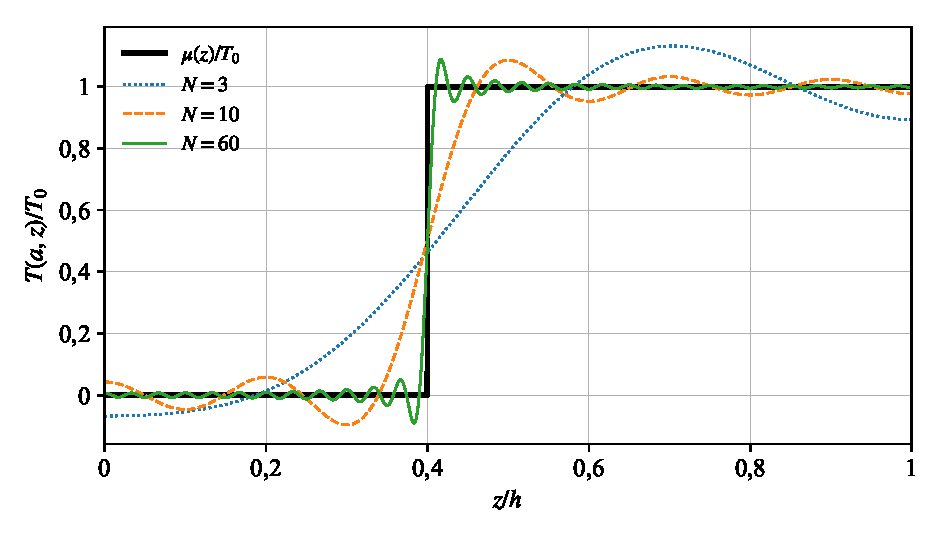
\includegraphics[width=0.92\textwidth]{fig_partial_sums}
  \caption{Функция $\mu(z)$ и частичные суммы ряда~\eqref{eq:solution}
  с $N$ слагаемыми при $r=a$, $c/h=0{,}4$}
  \label{fig:partial}
\end{figure}

Для численной проверки вычислены значения суммы ряда~\eqref{eq:solution}
(программа приведена в файле \texttt{code/analytic.py}). При
$a/h=0{,}5$, $c/h=0{,}4$ отклонение суммы $2\cdot10^4$ слагаемых от
$\mu(z)$ при $r=a$ вне промежутка $|z-c|<0{,}05h$ не превышает
$10^{-4}\,T_0$, в точке $(a,c)$ сумма равна $0{,}5000\,T_0$. Разностная
проверка подтверждает, что $T_{rr}+T_r/r+T_{zz}=0$ внутри цилиндра и
$\partial T/\partial z=0$ на торцах. Значение $T$ в точке
$r=0{,}6a$, $z=0{,}55h$, вычисленное по формуле~\eqref{eq:T-green}
численным интегрированием производной ряда~\eqref{eq:G}, совпадает
с суммой ряда~\eqref{eq:solution} ($0{,}7617\,T_0$).

\emph{Средняя по высоте температура.} Интегралы от
$\cos(\pi nz/h)$ по отрезку $[0,h]$ при $n\ge1$ равны нулю, поэтому
при любом~$r$
\begin{equation}
\label{eq:mean}
\frac{1}{h}\int\limits_0^h T(r,z)\,dz=T_0\Bigl(1-\frac{c}{h}\Bigr) .
\end{equation}
Физический смысл: тепловой поток через любую соосную цилиндрическую
поверхность радиуса $r<a$ равен
$Q(r)=-2\pi r k\int_0^h T_r\,dz=-2\pi rk\,\frac{d}{dr}\int_0^h T\,dz=0$.
Через верхнюю часть такой поверхности тепло идёт к оси, через нижнюю~—
от оси, и в сумме эти потоки равны нулю. Это же верно и для боковой
поверхности: сколько тепла входит в тело через горячий пояс $c<z<h$,
столько же уходит через холодный $0<z<c$.

\emph{Симметрия.} При $c=h/2$ слагаемые с чётными~$n$ равны нулю
($\sin(\pi n/2)=0$), а при нечётных~$n$
$\cos\bigl(\pi n(h-z)/h\bigr)=-\cos(\pi nz/h)$. Поэтому
$T(r,h-z)=T_0-T(r,z)$: распределение температуры антисимметрично
относительно середины высоты.

\emph{Предельные случаи.} Если цилиндр широкий ($a\gg h$), то при
$a-r\gg h$ по~\eqref{eq:ratio-asympt} все слагаемые ряда малы, и
$T\approx T_0(1-c/h)$: вдали от боковой поверхности температура равна
среднему значению~\eqref{eq:mean}. Если цилиндр узкий ($a\ll h$), то
отношения функций Бесселя близки к единице для всех $n\ll h/a$, и
$T(r,z)\approx\mu(z)$, сглаженной на участке длины порядка~$a$ около
$z=c$: температура в каждом поперечном сечении почти равна температуре
боковой поверхности на этой высоте.

\emph{Оценка числа слагаемых.} Из~\eqref{eq:ratio-asympt} следует, что
модуль $n$-го слагаемого не превышает
$\frac{2T_0}{\pi n}\sqrt{a/r}\,e^{-\pi n(a-r)/h}$. Чтобы погрешность
отбрасывания членов с номерами больше~$N$ была порядка~$\gamma\,T_0$,
достаточно взять
$N\approx\frac{h}{\pi(a-r)}\ln\frac{1}{\gamma}$ слагаемых. Чем ближе
точка к боковой поверхности, тем больше нужно слагаемых. Значения суммы
ряда при разном~$N$ приведены в таблице~\ref{tab:conv}.

\begin{table}[H]
  \caption{Значения $T/T_0$ по формуле~\eqref{eq:solution} при
  $a/h=0{,}5$, $c/h=0{,}4$ и разном числе слагаемых~$N$}
  \label{tab:conv}
  \centering
  \begin{tabular}{|c|c|c|c|c|c|c|}
    \hline
    $r/a$ & $z/h$ & $N=1$ & $N=2$ & $N=5$ & $N=10$ & $N=50$\\
    \hline
    0     & 0,4 & 0,49114 & 0,51878 & 0,51453 & 0,51451 & 0,51451\\
    0,5   & 0,4 & 0,47370 & 0,52119 & 0,51001 & 0,50979 & 0,50979\\
    0,9   & 0,4 & 0,42957 & 0,54698 & 0,50668 & 0,50303 & 0,50192\\
    0,5   & 0,1 & 0,21128 & 0,16379 & 0,17699 & 0,17740 & 0,17741\\
    0,5   & 0,9 & 0,98872 & 0,94122 & 0,93391 & 0,93410 & 0,93409\\
    \hline
  \end{tabular}
\end{table}

\section{Распределение температуры}
\label{sec:picture}

Распределение температуры, вычисленное по формуле~\eqref{eq:solution}
при $a/h=0{,}5$ и $c/h=0{,}4$, показано на рисунках~\ref{fig:iso}
и~\ref{fig:profiles}. На рисунке~\ref{fig:iso} изображено осевое сечение
цилиндра (правая половина~— прямоугольник~$\Pi$, левая~— его зеркальное
отражение относительно оси).

\begin{figure}[H]
  \centering
  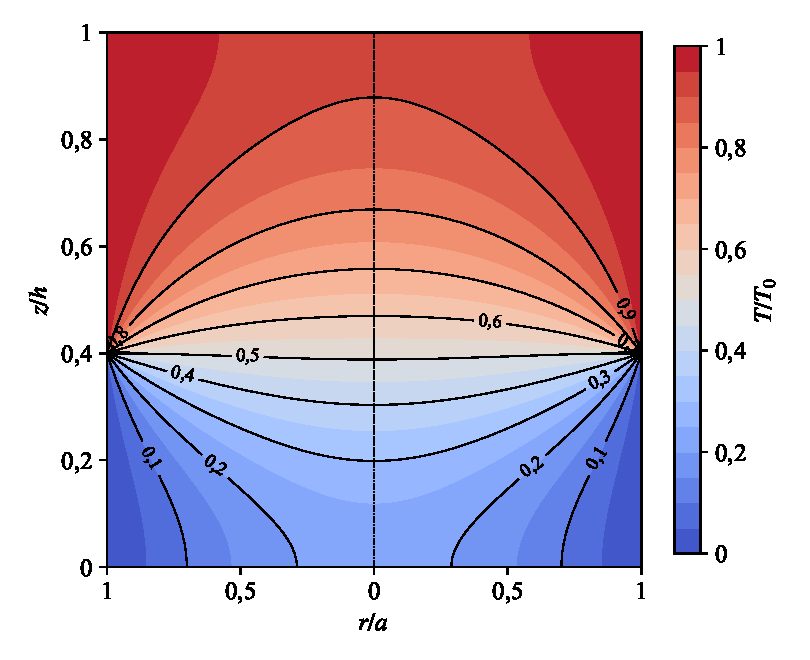
\includegraphics[width=0.8\textwidth]{fig_isotherms}
  \caption{Изотермы $T/T_0=\mathrm{const}$ в осевом сечении цилиндра,
  $a/h=0{,}5$, $c/h=0{,}4$}
  \label{fig:iso}
\end{figure}

\begin{figure}[H]
  \centering
  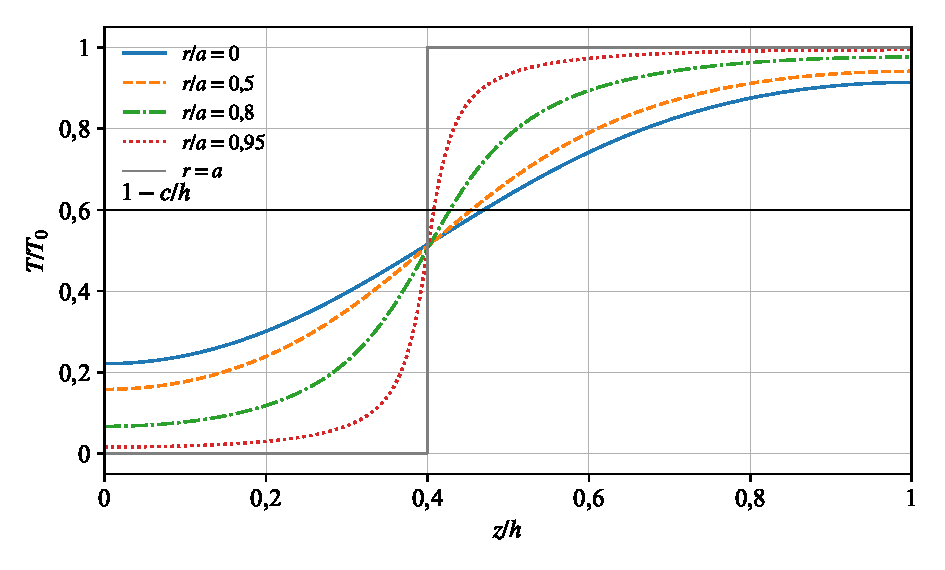
\includegraphics[width=0.92\textwidth]{fig_profiles}
  \caption{Распределение температуры по высоте цилиндра на разных
  расстояниях от оси, $a/h=0{,}5$, $c/h=0{,}4$}
  \label{fig:profiles}
\end{figure}

По рисункам видно следующее.
\begin{enumerate}
  \item Все изотермы с $0<T<T_0$ выходят из точки $(a,c)$, в которой
        граничная температура меняется скачком. Вблизи этой точки решение
        ведёт себя как $T\approx T_0\bigl(\tfrac12+\psi/\pi\bigr)$, где
        $\psi$~— полярный угол с вершиной в точке $(a,c)$, отсчитываемый
        от направления внутрь цилиндра. Поэтому изотермы около неё~—
        лучи, и в самой точке решение разрывно.
  \item Изотермы подходят к торцам под прямым углом: это геометрический
        смысл условия теплоизоляции $\partial T/\partial z=0$.
  \item Температура заключена между 0 и $T_0$, как
        следует из оценки~\eqref{eq:bounds}.
  \item По мере удаления от боковой поверхности к оси профиль
        температуры сглаживается: скачок $\mu(z)$ превращается в плавный
        переход, а на оси температура меняется лишь от $0{,}22\,T_0$ до
        $0{,}92\,T_0$.
  \item Все профили на рисунке~\ref{fig:profiles} имеют одно и то же
        среднее значение $1-c/h=0{,}6$, как следует из~\eqref{eq:mean}.
  \item Изотерма $T=T_0/2$ изогнута вниз от точки $(a,c)$: так как горячий
        пояс длиннее холодного ($h-c>c$), на оси на высоте $z=c$
        температура $0{,}5145\,T_0$ больше $T_0/2$.
\end{enumerate}

Подробный анализ зависимости решения от параметров $a/h$ и $c/h$
и сравнение с численным решением выполняются в следующих разделах отчёта.
   % 3 Аналитическое решение          (этап 2)
% \input{chapters/ch4} % 4 Численное решение
% \input{chapters/ch5} % 5 Анализ полученных решений
% \input{conclusion}   % Выводы
% ============================================================
% refs.tex — СПИСОК ИСПОЛЬЗОВАННЫХ ИСТОЧНИКОВ
% Порядок — по первому упоминанию в тексте (ГОСТ 7.32-2017, п. 6.16)
% ============================================================
\chapter*{СПИСОК ИСПОЛЬЗОВАННЫХ ИСТОЧНИКОВ}
\addcontentsline{toc}{chapter}{СПИСОК ИСПОЛЬЗОВАННЫХ ИСТОЧНИКОВ}

\begin{enumerate}[wide=\parindent, label=\arabic*., nosep]

  \item Куликов~К.\,Г., Фирсов~А.\,Н.
    Уравнения и методы математической физики. Классические модели~:
    учеб. пособие / под ред. В.\,Н.~Козлова.~---
    СПб.~: Изд-во Политехн. ун-та, 2011.~--- 220~с.

  \item Тихонов~А.\,Н., Самарский~А.\,А.
    Уравнения математической физики~: учеб. пособие для вузов.~---
    5-е изд., стер.~--- М.~: Наука, 1977.~--- 735~с.

  \item Смирнов~В.\,И.
    Курс высшей математики. Т.\,2.~---
    21-е изд., стер.~--- М.~: Наука, 1974.~--- 656~с.

\end{enumerate}

\clearpage

\end{document}
